\chapter{16 Tales - Volume 3}

\begin{figure}[H]
    \centering
    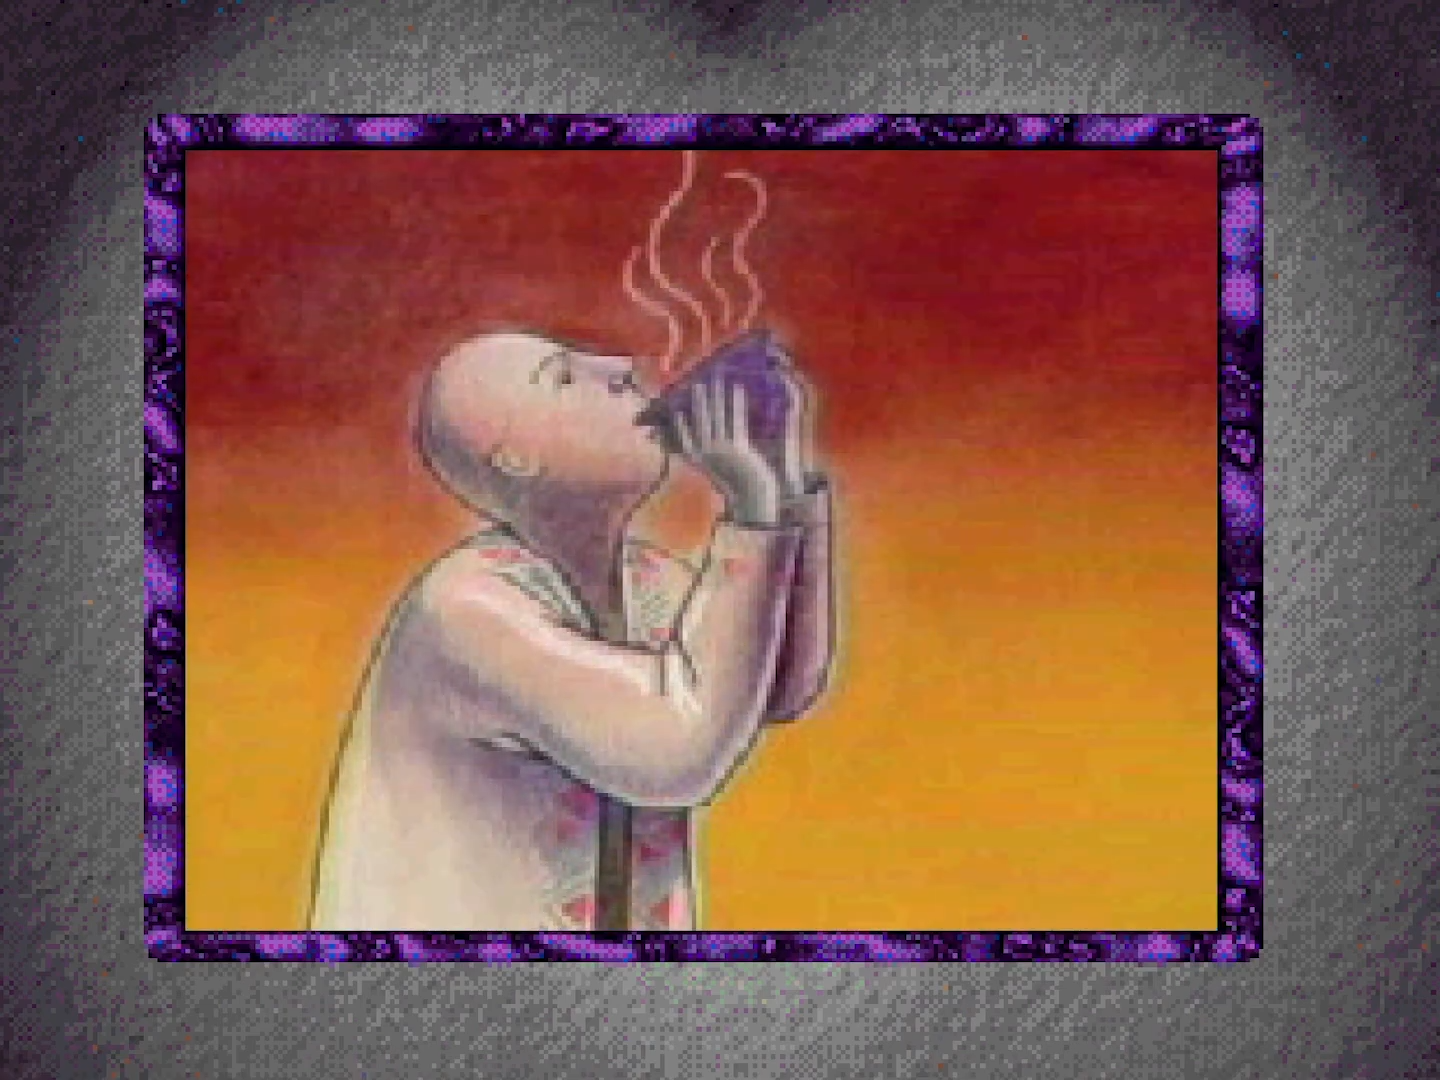
\includegraphics[width=\textwidth/2]{"./Games/16Tales/Images/16Tales3Screenshot.png"}
    \caption{16 Tales 3 Screenshot}
\end{figure}

The third of the four 16 Tales games published and released by The Lightspan Partnership for the PlayStation 1.

16 Tales - Volume 3 features four 15-minute video programs detailing the following Spanish and Latin American stories:

\begin{itemize}
    \item The Flea
    \item The Lazy Fox \& Señor Coyote and Señor Fox
    \item Tepozton, the Magic Boy from the Mountains
    \item The Tiger and the Rabbit
\end{itemize}

Music used throughout:
- Sun Valley by David Snell

\begin{table}[h]
    \centering
    \begin{small}

        \begin{tabular}{|p{1.5cm}|p{8.5cm}|p{7cm}|}
            \hline
            \textbf{Story Title} & \textbf{Short Description} & \textbf{Credits} \\
            \hline
            The Flea
                                 &
            In this story, the narrator discusses the nature of folk tales and their origins, emphasizing their simplicity and longevity.
            The tale of "The Flea" originates in Spain, where a king, fond of riddles, captures a flea and decides to raise it as a royal pet.
            He concocts a riddle involving the flea as a test for suitors seeking to marry his daughter.
            Many fail, facing dire consequences, until a poor shepherd, aided by a mouse and an ant, cleverly solves the riddle and wins the princess's hand.
            The story concludes with a moral about the value of friendship and resourcefulness, and encourages readers to explore more folk tales and even create their own stories.
                                 &
            Told by: Pedro Martinez,
            Producer: K. Hamamura Nelson,
            Executive Producer and Director: Edmond R. Chavanette,
            Story Editor: Severo Perez,
            Illustrator: Steven A. Garcia,
            Titles and Set: Doug Stiles,
            Lighting: Ron A. Vanicek,
            Technical Director: Bill Bolle,
            Audio: Larraine E. Wilson,
            Video: Roger Knipp,
            Videotape: Clarence Pemberton,
            Camera: John C. Merritt, Martin Miller, Ron A. Vanicek,
            KLCS Los Angeles Unified School District
            \\
            \hline
            The Lazy Fox \& Señor Coyote and Señor Fox
                                 &
            In "The Lazy Fox," a clever fox tricks an armadillo into doing all the work on his farm by offering to share the harvest.
            However, the fox's plan backfires when the armadillo cleverly plants crops that leave the fox with only the undesirable parts.
            The fox's attempts to change the terms of their agreement fail, and he ends up empty-handed.
            In "Señor Coyote and Señor Fox," a coyote encounters a sleeping fox near a cliff and is tricked into holding up the cliff to prevent it from falling.
            The fox promises to get help but never returns, leaving the exhausted and deceived coyote alone.
            These stories, originating from Argentina and Mexico, respectively, highlight themes of cunning and deception, showcasing the wit of the characters involved.
            The narrator encourages readers to explore more folk tales from around the world, emphasizing the richness and diversity of storytelling traditions.
                                 &
            Told by: Pedro Martinez,
            Producer: K. Hamamura Nelson,
            Executive Producer and Director: Edmond R. Chavanette,
            Story Editor: Severo Perez,
            Illustrator: Rick Tejada-Flores,
            Titles and Set: Doug Stiles,
            Lighting: Ron A. Vanicek,
            Technical Director: Bill Bolle,
            Audio: Larraine E. Wilson,
            Video: Roger Knipp,
            Videotape: Clarence Pemberton,
            Camera: John C. Merritt, Martin Miller, Ron A. Vanicek,
            KLCS Los Angeles Unified School District
            \\
            \hline
            Tepozton, the Magic Boy from the Mountains
                                 &
            The story "The Tale of the Magic Boy" is set in ancient Mexico and revolves around a boy named Tepo Stone, who is believed to have divine origins.
            Born to a god and a mortal woman, Tepo Stone is placed in a box and sent down a river, where he is found by an elderly fisherman and his wife.
            As Tepo Stone grows up, he displays extraordinary abilities, including shooting arrows that change direction in mid-air.
            When his village is threatened by an evil giant who demands human sacrifices, Tepo Stone volunteers to be the sacrifice, ultimately outsmarting the giant and becoming a hero.
            He later discovers his true heritage and goes to live with his godly father.
            The story concludes with the suggestion that Tepo Stone may still be among the people, living as an ordinary person.
            It encourages readers to explore other tales of magic and adventure from Mexico and beyond.
                                 &
            Told by: Rose Portillo,
            Producer: K. Hamamura Nelson,
            Executive Producer and Director: Edmond R. Chavanette,
            Story Editor: Severo Perez,
            Illustrator: Joanna Cooke,
            Titles and Set: Doug Stiles,
            Lighting: Ron A. Vanicek,
            Technical Director: Bill Bolle,
            Audio: Larraine E. Wilson,
            Video: Roger Knipp,
            Videotape: Clarence Pemberton,
            Camera: John C. Merritt, Martin Miller, Ron A. Vanicek,
            KLCS Los Angeles Unified School District
            \\
            \hline
            The Tiger and the Rabbit
                                 &
            The story "The Tiger and the Rabbit" is set in Puerto Rico and reflects the island's cultural diversity with influences from the Arawaks, Spaniards, and Africans.
            It tells the tale of a clever rabbit and a foolish tiger.
            Despite the tiger's attempts to catch and eat the rabbit, the rabbit outsmarts him at every turn, eventually leading to their unlikely friendship.
            Through a series of humorous encounters, the rabbit tricks the tiger into embarrassing situations, showcasing the rabbit's wit and the tiger's gullibility.
            The story concludes with the tiger and the rabbit becoming friends, although the tiger's hunger remains a constant threat to their relationship.
            It encourages readers to explore more tales from Puerto Rico and around the world.
                                 &
            Told by: Rose Portillo,
            Producer: K. Hamamura Nelson,
            Executive Producer and Director: Edmond R. Chavanette,
            Story Editor: Severo Perez,
            Illustrator: Joanna Cooke,
            Titles and Set: Doug Stiles,
            Lighting: Ron A. Vanicek,
            Technical Director: Bill Bolle,
            Audio: Larraine E. Wilson,
            Video: Roger Knipp,
            Videotape: Clarence Pemberton,
            Camera: John C. Merritt, Martin Miller, Ron A. Vanicek,
            KLCS Los Angeles Unified School District,
            \\
            \hline
        \end{tabular}
    \end{small}

\end{table}

\clearpage
\newpage

\section{Transcriptions}

\subsection{The Flea}
Folk tales are old, simple, and not too hard to remember. Many are stories that were told long before the invention of printing. They were passed on by word of mouth. Now, if a story is repeated enough times, and if its meaning is lasting, it may be on its way to becoming a folk tale, even if it's make-believe, like the story you'll hear today.

The Flea is a story from Spain. Spain, like other countries in Western Europe, has retained many of its customs and traditions of the past. Spain is famous for its beautiful old castles which can still be seen on the hillsides and in the older cities.

Today, many of the Spanish people live in large cities like Madrid and Barcelona. They live in modern homes and apartments, and life in the city is like life anywhere else, but the country life has not changed as much.

Farmers live in small villages and towns and tend fields much as they did in the days of long ago. The people still have a king; however, he is more like our president than the king in our story.

The Flea is a tale that shows that people are very much alike all over the world because we like to laugh at ourselves and at others. We cook up explanations for things we don't really understand, and sometimes we just make talk about our everyday lives. [Ahora y gochemos]. Listen to the tale of the Flea.

    [Eva, una vez en España]. There was once a king of Spain who loved riddles. It just delighted him to ask one that no one could answer, so of course, he spent many hours thinking of new riddles.

One day, as the King was being dressed by his servants, a flea jumped from one of the pages onto the king. The king snapped it up in his fingers and called for his Chamberlain.

"Chamberlain, what is this?" demanded the king.

The Chamberlain was very embarrassed when he saw what was in the king's hand. "Oh dear, it's a flea," he said in a low voice.

"A flea?" said the king. "Does the king of Spain have fleas?"

"Oh no, your highness, I must be mistaken. That cannot be a flea," begged the Chamberlain.

"Of course it's a flea!" shouted the king. "But because it has landed on me, it is a royal flea. Now, I wonder what I should do with it."

The poor Chamberlain shrugged his shoulders as the king pondered over the flea.

At last, the king said, "I know! We shall put this flea in a cage worthy of a royal flea, and we shall feed it royal food. I want this flea to grow as big as a cat. No, no, let me see... bigger than that, as big as a goat. No, even bigger than that! I want this flea to be as big as an elephant! Then, I shall have the flea skinned to make a tambourine for my daughter, Belita."

The King was so excited he shook with laughter. "Don't you see, Chamberlain?" said the King. "This is truly a riddle worthy of a king. Every suitor that comes to ask for my daughter's hand in marriage shall be asked the riddle. The one who answers it correctly shall marry my daughter, and I think I shall name this flea Felipe."

The Chamberlain looked at the little flea and wondered to himself if the king had gone mad.

Every day for the next six months, the king visited Felipe to check on her progress. Well, at the end of the first month, the flea was as big as a mouse, and the following month, as big as a cat. By the sixth month, she was as big as a goat, and the King could wait no longer. He ordered that the flea skin be made into a tambourine. Then, he had the Royal dance instructor teach Belita to dance with her tambourine, and the King composed a riddle. It went like this: "Belita, Felipe, they look so well together. Belita, Felipe, if you can only answer whether what animal is Felipe, what animal is Felipe, if you can tell about Felipe, you then can marry Belita."

Well, soon the king grew tired of this business since no one could answer the riddle. Every day, more young men arrived to waste his time. So the king commanded that any suitor who could not guess the riddle would have his head cut off. Of course, all of the suitors disappeared. Belita, it seemed, was destined to live the rest of her days as an Old Maid.

At this time, far away in the Castilian Hills, there lived a shepherd. He was young and handsome, but he was as poor as the poorest beggar in all of Spain. One day, the shepherd thought to himself, "I have nothing to lose; perhaps I should try to answer the riddle." So he said goodbye to his mother and his brother. His mother gave him a small pouch filled with cheese, and his brother gave him a walking staff, and then they sent him on his way.

Well, the shepherd had not gone far when he heard a tiny voice shout, "Stop! Stop!" The shepherd stopped and looked around, and there on the ground was a small black ant.

"Thank you for not stepping on me," said the ant. "I am very grateful."

The shepherd told the ant he was on his way to the king's Palace, and the Ant immediately said, "Please take me with you. I have always wanted to see the king's Palace."

"But I can't carry you," said the shepherd.

"How about your pouch?" said the ant.

"I have cheese in my pouch," answered the shepherd, "and you would get it all dirty."

"Oh, but I'll wipe my feet," said The Ant, "and I promise not to step on your cheese." So the shepherd put the ant in his pouch and walked on.

He walked all day, and in the evening, he slept by a small stream. In the morning, when he awoke, he heard a small voice calling, "Help! Help!"

The shepherd looked around, and in the stream in front of him, he saw a mouse thrashing about in the water. He reached into the water with his staff and saved the mouse.

"Thank you, thank you for saving my life," said the mouse. "How can I repay you?"

"There's no need for that," said the shepherd. "I'm on my way to the king's Palace to try and answer the riddle. If I can't answer it, I shall have my head cut off, and if I do answer it, I shall be rich."

"Well then," said the mouse, "can you take me with you to the Palace?"

"But I have no place to hide you," replied the shepherd.

"You have a pouch," said the mouse.

"But I have my breakfast inside the pouch. There is not enough room for you too."

"If you ate your breakfast now, there would be plenty of room," begged the mouse.

It was true, and the shepherd was hungry, so he took out the cheese and gave a small piece to the mouse and a smaller piece to The Ant, and after they ate, they continued on their way.

When the shepherd arrived at the palace, he became frightened, so he sat under a tree to try to regain his courage.

"What's wrong?" asked the mouse.

"The thought of losing my head is not very pleasant," said the shepherd.

"Come on, we will help you," said the mouse. So the shepherd went up the palace stairs and said he had come to answer the riddle.

When he saw the shepherd, the Chamberlain gasped. "It's not too late to turn back," he said, but the shepherd was determined and was finally presented to the king.

The king took in the sad sight of the poor Shepherd and said, "Our Shepherd's life is better than no life at all." But the shepherd insisted on answering the riddle, so Belita danced, and the King repeated his riddle: "What animal is Felipe, what animal is Felipe? If you can tell about Felipe, you then may marry Belita."

When the dance was over, the Shepherd studied the tambourine carefully and knew right away it was not the skin of a sheep.

"Can you guess what it is?" said the ant.

"No, I can't," replied the shepherd sadly.

"Quickly, let me out of the pouch. Maybe I can help," said the ant.

The shepherd took the ant out of his pouch, and the ant crawled all over the tambourine.

"There is no mistaking it," said the ant softly. "It is a flea."

"Are you sure?" said the shepherd.

"Absolutely," replied the ant.

"Oh, stop muttering to yourself," said the king. "Quickly, answer the question."

"Felipe is a flea," said the shepherd. Oh, the court was all in a flutter!

"I can't marry a poor Shepherd," cried Belita.

"And you certainly shall not," said the king.

"But you gave your word," said the shepherd.

"It's just that you are so poor," said the king. "How could you possibly care for my daughter? Instead, I will grant anything you wish. Just name it, and it's yours."

"Ask him to fill your pouch with gold," whispered the mouse.

"Well then, um, I would like to have my pouch filled with gold," said the shepherd.

"That's easy enough," said the king. "Quickly, bring some gold," he commanded.

The Chamberlain arrived with the gold, but the mouse had gnawed a hole in the bottom of the pouch, and the gold poured right through. The Chamberlain went to get more gold, and then more and more, because the pouch was never full.

Finally, the shepherd said, "Enough! Now I am a rich man. I can support your daughter in any manner she wishes."

And so it was, the Shepherd married a princess and lived a long, comfortable life. The Mouse and the Ant lived happily too, for the shepherd never forgot how they had helped him.

    [Y colorín colorado este cuento se acabo]. The Spanish people have a special love for friendly animals, among their favorites are two who appeared in this story: [La Hormiguita], the little ant and [El Raton], the mouse.

Now, a make-believe story like The Flea is a fairy tale, but other animal stories which teach people how to live are called fables. Read and enjoy folk tales from Spain and from all over the world. You can find them in your school or public libraries, or make up a story of your own. [Y colorín colorado este cuento se acabo.] Share a story with a friend, so our tales will never end.

\subsection{The Lazy Fox \& Señor Coyote and Señor Fox}

Today, you will hear two stories: first, The Lazy Fox, and then the story of Señor Coyote and Señor Fox.

Our first story, The Lazy Fox, is from Argentina. Argentina. Argentina is the second-largest country in South America. The character of the fox was brought to South America in stories carried by the Spanish explorers of long ago. You see, the fox is a character often found in the folk tales of Spain. The Lazy Fox tries to outwit the hard-working armadillo. The armadillo is an animal found only in the American continents. So, in this story from Argentina, we'll see a blending of European and South American cultures.

Señor Coyote and Señor Fox is a story from northern Mexico. In Mexico, there are many stories about Coyote, a character borrowed from Indian folklore. Coyote is very clever and can usually get the best of anyone. [Ahora y gochemos.]

Listen now to the tales of The Lazy Fox and Señor Coyote and Señor Fox.

Once, there was a fox who was very well-known for the tricks he played on everyone. This fox owned a farm, but he never did any work on it. He would lie around all day long in the coolest shade.

One day, he looked out at his field and wondered how he could get someone to plant and harvest it for him. "All day long, that armadillo works in the hot sun on that rock patch he calls a farm. Why, it should be easy to talk someone so stupid into doing all my work for me. At the end of the harvest, I'll even give him a share, but just a small one."

The fox hurried over to the armadillo's farm and found him working in the field. "Ah, good morning. How is it going?" called the fox.

The armadillo looked up and said, "Not very well. You know, this land is so rocky, I have to be very careful, or I'll break my plow."

"Well," said the fox, "I think I can help you."

"Me?" said the armadillo. "How can you help me?"

"You know, I have a very nice piece of land. If you would only plant it for me, I would ask for only a small share in payment."

"Why are you so generous?" asked the armadillo.

"Oh, this has been a very good year for me," said the fox, "and I've decided to let others share in my good fortune."

"That's very kind of you," said the armadillo as he leaned back on his hoe. "What kind of crop do you want to plant?"

"Anything you want to plant," said the fox, "and I'll let you have half of the crop..."

"Half?" said the armadillo.

"Better yet, I'll let you have anything that grows above the ground, and I'll keep what grows below the ground."

Now, the fox knew the armadillo loved potatoes, so he just assumed that would be the armadillo's choice.

"That sounds fair to me," said the armadillo, and they shook hands on their agreement.

The next day, the armadillo and his family got up early and went to work on the fox's field.

When the fox finally got around to checking on their work, it was nearly sunset.

"How is it going?" shouted the fox.

"We're almost through planting," answered the armadillo, "but it looks like rain, so we'd better hurry and finish up today."

The fox looked up and saw the clouds gathering, so he hurried away without asking what it was they were planting.

Well, the crop grew and grew, and at last, it was time to harvest the crop. The armadillo family arrived early in the morning, and by noon, they had harvested a fine crop of wheat.

Well, the fox didn't get up until midday, so when he went out to the field to collect his share, all that remained was the shriveled, tasteless roots. Oh, the fox was furious! He raced right over to the armadillo's house, and when he got there, he found the family eating bread.

"There's been a terrible mistake," said the fox.

"What's the problem?" said the armadillo. "Didn't we keep our part of the agreement?"

"Yes, of course you did, but uh... I thought..." The fox was going to say he thought they were going to plant potatoes, but he didn't. Instead, he said shrewdly, "I thought you liked roots."

"I do," said the armadillo.

"Well, next season, I want everything that grows above the ground," said the fox.

"That sounds fair to me," answered the armadillo.

The fox went away with his stomach grumbling. He had planned to trick the armadillo out of the entire harvest, and now he had nothing to eat.

Again the next season, the armadillos diligently worked the field. The fox didn't bother to show up until the day of the harvest, and on that day, he didn't arrive until noon. By then, the armadillos were on their way home, and all that was left were the tops of the potato plants the armadillo had planted.

"Come back!" hollered the fox. "I think you're trying to trick me!"

"But that's what we agreed, isn't it?" replied the armadillo.

"You never think of me when you plant," said the fox. "Next season, I want the tops as well as what grows under the soil. You can have all that grows in the middle."

"Well, I don't know," said the armadillo.

"I think it's only fair. I didn't get any of the first two crops," demanded the fox.

The armadillo was silent for a moment, and then said, "All right, I think it's fair too."

And the fox went away with his stomach grumbling again. He looked at his shadow and thought, "Oh, how thin I'm getting!" But this time, he felt certain there was no way the armadillo could get any of the crop, and at least that made him feel a little better.

The next harvest, the fox arrived early in the morning to find the Armadillo had planted corn. The crop was large, and the ears were especially succulent, but they grew right in the middle of the plant.

"You have tricked me again," said the fox.

"How could that be?" said the Armadillo. "We gave you just what you asked for."

The Hungry Fox watched the armadillo haul away the corn harvest. "That's the last time I'm going to let you use my fields!" he shouted. The armadillo didn't say anything, he just walked away slowly because not only was the crop heavy, but he had put on a lot of weight over the last three seasons.

Now, on another day in a desert not too far away, the coyote was looking for something to eat. He saw a large Mesa in the distance, and he thought he might find a small animal sleeping in the shade of the cliff.

When he arrived by the edge of this great cliff, he began looking around, but instead of a tasty little animal, he found his old enemy, the fox, sleeping as usual.

"Here's my chance to get that fox," thought the coyote. The fox, however, never sleeps like other animals. He sleeps with one eye open.

So when he saw his enemy, the coyote, sneaking up on him, the fox jumped to his feet and began pushing hard against the rock cliff. "Help me!" he shouted at the coyote. "Please help me, or this cliff will fall on us and kill us both!"

The coyote was a bit confused. He looked at the fox straining and pushing against the rock cliff like his life depended on it.

"See for yourself," said the fox. "The cliff is falling!"

The coyote looked up. Up, up to the top of the cliff, and sure enough, it looked as if it were going to fall over on him. He jumped to the cliff wall next to the fox and began pushing with all his might.

"That certainly was close," said the fox. "I'd certainly be dead if you hadn't come along."

The coyote looked up again and saw that it was still falling, so he pushed very hard, so hard that he was kicking up ground with his feet.

"We're doomed," said the fox sadly. "We will probably die here together."

"No, we won't," said the coyote. "Help will come soon enough."

"No, we are the only ones here, and no one ever comes this way." The coyote looked up only to scare himself again and pushed even harder against the cliff.

"I've got an idea," perked up the fox. "There may be a way out of this."

"What's that?" grunted the coyote.

"I'll go get help, and you stay here and hold up this cliff," said the fox.

"Why don't you hold up the cliff, and I'll go for help?" asked the coyote.

"Well, you are more than twice as strong as I am and can surely hold it up by yourself. I'll be back in just a few minutes."

"All right," replied the coyote, "but hurry!"

"Push harder, harder!" called the fox as he ran away.

The coyote pushed and pushed. His arms and legs hurt so badly he thought they would break. A few minutes became an hour, an hour became two. The coyote pushed so hard he began to dig a hole in the ground with his feet. The day passed, the sun set, night came. Oh, it was cold and dark!

The coyote shivered and called out for the fox, but the fox didn't come. When the sun finally rose, he was so tired he was quivering. "I can't last much longer," he gasped. Tears were rolling down his face. "This is the end," he thought. "I might as well try to make a run for it because if I stay, I will die anyway."

He gave one last shove, and with all the strength he had left, he ran away from the cliff. When he looked back, he saw the Mesa still standing. He blinked, he rubbed his eyes. It wasn't going to fall, not now, not in a hundred years! He had been tricked! The fox was nowhere to be found. He was napping in some dark, cool place far away.

    [Y colorín colorado este cuento se acabo]. These are just two stories which have been translated from Spanish. There are hundreds of others. You can find stories from Mexico and Argentina, and from all over the world, in your school or public libraries. Read and enjoy the folk tales of the world. [Y colorín colorado este cuento se acabo] Share a story with a friend, so our tales will never end.

\subsection{Tepozton, the Magic Boy from the Mountains}

Today's story, The Tale of the Magic Boy Tepo Stone, was told by the Indians who built their cities in the valleys of ancient Mexico.

In Mexico, there are two huge mountain ranges: the Sierra Madre Occidental and the Sierra Madre Oriental. It was here that the Azteca, the Mixteca, the Tolteca, and other Indians built their magnificent cities all of stone.

Now, since the mountains surrounding the city were always covered by clouds, the people believed that the mountaintops must be the home of the Gods. Stories of the gods and their magic are told in Mexico even today, in the modern cities as well as in the smaller villages.

    [Ahora y gochemos.] Listen now to the tale of Tepo Stone.

A long, long time ago, before anyone who is alive today can remember, there lived a little boy named Tepo Stone. He lived with an old fisherman and his wife in a house by the river. Tepo Stone thought the old fisherman and his wife were his real parents, but his real father was a god, a God who lived in a giant volcano high above the clouds.

In those days, the Gods had their jobs to do. They controlled the winds and made the rain fall at the right time so that the crops would grow. The gods discovered many things which they taught to the people.

But one of the Gods got tired of living in the volcano and decided it would be nice to have a wife and child. So he came down from the fiery volcano to be with people. While stopping by a stream, he saw a beautiful girl picking flowers, and right away, they fell in love. So he gave her a green stone, and with that, they were married.

After a while, she gave birth to a son. Now, one day, the God decided he had to return to his Mountain to make the rain fall and control the winds. This made his wife very sad because the laws of her people would not allow a mother to keep a fatherless child.

Well, before anyone could take away her child, she put him into a box, and around Tepo Stone's neck, she tied the smooth green stone given to her by the God, and she let him float down the river. And that is how the fisherman and his wife came to find the little baby boy. The Box floated down the river and stopped in the shallow water in front of their house.

Well, the fisherman and his wife were very happy, for they had wanted children for a long time and couldn't have any.

"What shall we call him?" said the fisherman.

His wife said, "Well, he has a green stone around his neck. You know, it reminds me of the green stones brought down from the mountains."

"Then we shall call him Tepo Stone, the boy from the mountains."

So that's how he got his name. Tepo Stone grew up strong and happy with his new parents. They loved him very much and took very good care of him.

When Tepo Stone was seven years old, the fisherman made him a bow with little arrows to go with it. "Now I will bring home all the food, and you can stay home and rest," said Tepo Stone.

The old fisherman laughed. "You are just a little boy," he said.

"But I can shoot anything I want," answered Tepo Stone.

"All right," said the fisherman, "shoot that Quail over there."

Well, Tepo Stone picked up his bow and placed an arrow to the string. He let the arrow fly in the wrong direction, but the arrow turned around in flight and killed the quail.

"There must be a wind," said the old man. "That could never happen twice. See that wild turkey on that tree? Let's see if you can hit him." The old man knew it was impossible to shoot the turkey at such a long distance.

But Tepo Stone fitted an arrow to the bow and again shot it in the wrong direction. Again, the arrow turned, and the turkey fell dead.

Well, from that day on, Tepo Stone did all the hunting, and the old fisherman and his wife stayed at home. He left before sunrise each day and returned just after sunset. And when the fisherman's wife asked him, "Tepo Stone, what do you do all day?" Tepo Stone would reply, "I have many things to do."

Well, one day, Tepo Stone was walking along a trail when he heard some men talking about an evil giant that lived in the woods. The giant had to be fed a human being every spring. Each year, he went to a new village and demanded that someone be handed over to him, or he would kill everyone in the entire village. Well the people were very scared of the giant, so they always obeyed him and selected someone to be eaten.

Tepo Stone also learned that this year, it was the Old Fisherman's Village's turn to supply a human being for the Giant. When he arrived home, the old fisherman was very sad. There were only three people he could send: himself, his wife, or Tepo Stone.

Well, so of course, he decided to go himself. The old fisherman did not tell Tepo Stone about his decision, but when the people arrived to take him away, Tepo Stone knew what they were there for.

"I won't let you take him away," said Tepo Stone to the people. "He's very old, and he won't make a good meal. I'm young and tender and will be much more satisfying to a hungry Giant."

The old fisherman would not hear of it. "You are young and have your life before you. I am old. I will die happy knowing you are well."

"But nothing will happen to me if I go," said Tepo Stone. He begged and begged the old man to believe him. Finally, the fisherman agreed and told him he could go.

Well, Tepo Stone immediately began to build a fire by the river. "Watch this fire," he told the fisherman. "As long as you see white smoke, you will know I am all right. But if the smoke turns gray, it will mean I am in danger, and if it turns black, it will mean I am dead." He assured the old man and his wife that he would return, and he went off with the people.

Now on the way to the Giant, Tepo Stone stopped and picked up shiny black stones, the kind used to make arrowheads and knives. His pockets were filled with them by the time they reached the Giant's Castle.

"What is this?" said the Giant. "How am I to feed on such a tiny morsel?" Oh the giant was huge. He was taller than 10 men standing on top of each other. "You bring me another," roared the Giant.

"Oh, I am little, but I taste very good," said Tepo Stone. "Why don't you try me and see?"

So the people brought in a large pot of boiling water, and Tepo Stone very willingly hopped in. The people then put the lid on the pot and went away. The giant went to sleep as his meal cooked.

A little later, the giant woke up and said, "Oh, I'm hungry. The boy is small, he must be cooked by now." But instead of a tasty little boy, there was a giant black leopard in the pot! The giant quickly put the lid back on the pot and went back to sleep.

When he woke up later, he was hungrier than before. But this time, the giant very carefully lifted the lid. While inside the pot, there was a huge snake! The snake hissed at the giant, so the giant put the lid back on the pot and went back to sleep.

The next time the giant woke up, he was so hungry he would eat anything. He didn't care what it was. He went over to the pot, took off the lid, and there was the little boy smiling at the Giant.

Well, this made the giant really angry, so he picked up the pot and swallowed all of its contents in one gulp. At that very moment, the smoke from the fisherman's fire turned from white to gray.

Oh, the old woman cried, and the old fisherman moaned. "He's only a little boy. I shouldn't have let him go."

Oh, but Tepo Stone was all right. You see, the giant had swallowed him whole, and he was sitting in the giant's stomach. Tepo Stone reached into his pocket and took out the stones he had collected along the way. He took two of them and hit them together so hard they broke in half. The edge of each one of the stones was as sharp as a razor.

Tepo Stone began to cut himself out of the giant's stomach. He cut and cut and cut. "Oh," the giant groaned. "I think I have heartburn."

And Tepo Stone kept on cutting and cutting. Well, by now, the hole was so large he could see daylight. Finally, he cut right through to the outside. Tepo Stone hopped out of the Giant, and all the people standing around cheered. At that moment, the smoke at the fisherman's fire, it turned from gray to white.

Tepo Stone then moved into the Giant's Palace and was soon crowned King. After a while, he learned about his real father, the God, and so he went to live with him.

Some say that he has returned and lives with the people, except no one knows who he is because he looks just like an ordinary person.

    [Y colorín colorado este cuento se acabo]. This story of Tepo Stone is just one of the many tales about the magic boy of the mountains. You can find others in your school or public library, stories like "How Tepo Stone Hung the Bells" and "The Magic Grocery Store." Read and enjoy other stories from Mexico and all over the world.  [Y colorín colorado este cuento se acabo]. Share a story with a friend, so our tales will never end.

\subsection{The Tiger and the Rabbit}

Our story today, "The Tiger and the Rabbit," comes from Puerto Rico, an island in the Caribbean Sea. Puerto Rico is a Spanish name which means "Rich Port."

Puerto Rico is a territory of the United States of America, and its people are United States citizens, but they have their own government.

Now, the first people to live here were the Indians called Arawaks. Later, Spaniards and Africans settled on the island, so today, Puerto Rico reflects the contributions of all three cultures.

The Spanish heritage of Puerto Rico is seen in the language and customs of its people. Spanish is the main language, although many Puerto Ricans also speak English.

"The Tiger and the Rabbit" is an animal story, and people everywhere love stories about animals. Stories from Spain tell about small animals that defeat mighty ones, and a little animal may be a mouse or an ant, but in Central America, it's often the rabbit. You see, the character of the rabbit was brought to Puerto Rico in the African tales of long ago.

    [Ahora y gochemos.] Listen now to the tale of "The Tiger and the Rabbit."

[Hace mucho tiempo]. Long, long ago, all the animals were friends and lived at peace with one another, that is, except for the tiger. The tiger liked to eat small animals, and his favorite meal was the rabbit. The rabbit, for this reason, became very clever and quick-witted. In fact, the rabbit thought the tiger was a stupid, clumsy fool. Even so, he always tried to stay out of the Tiger's way.

One day, the rabbit was playing his guitar under the shade of a tree. Along came the tiger and crept up on the rabbit. Well, before the rabbit could get away, the tiger jumped and grabbed him.

"Aha, now I've caught you," said the Tiger.

The little rabbit pretended not to be scared and answered calmly, "Ah well, tiger, you've come along at the right time. I was just sitting here playing my guitar and thinking about the best way to die, and if you knew what was going to happen, you would not care to live either."

"What's going to happen?" asked the Tiger.

"Oh, hurry, eat me and be done with it," said the rabbit. "You will need all the strength you can get."

"But what's going to happen?" demanded the Tiger.

"You mean you haven't heard?" said the rabbit. "There's a hurricane coming, and it's worse than any we've ever had. They say that all the animals will be washed away."

"Oh, that's terrible!" cried the Tiger. "What am I going to do?"

"For you, there's hope," said the rabbit. "You can tie yourself to a good strong tree, but for me, it's hopeless."

"Tie myself to a tree?" whimpered the Tiger.

"Sure, this one will do. It's withstood several hurricanes and will certainly stand another."

"Oh, thank you, thank you for helping me," said the tiger. "I don't want to be washed away."

So the rabbit tied the tiger to the tree. Then he climbed up the tree to keep his eye on the tiger.

Just then, a small herd of goats came walking down the road. When they first saw the tiger, they were frightened, but then they noticed the tiger was tied to the tree, and they laughed and laughed.

"You wouldn't be laughing if you knew what was going to happen," said the Tiger.

"Oh really, what's going to happen?" asked the goats.

"A hurricane is coming, and it's going to wash all of us away."

"A hurricane?" said the goats. "We haven't heard of a hurricane."

The goats talked among themselves and finally said to the Tiger, "We have come from the mountains and across the hills, and no one has mentioned such news. There's no hurricane coming."

The tiger knew at once he had been tricked, and the sight of the fat little goats made him even more angry because he was hungry.

"Well then, why don't you untie me?" said the Tiger.

But the goats just laughed and ran away. Well, what could be funnier than a tiger tied to a tree?

Oh, the tiger struggled and struggled, but he only got more and more tangled.

In a while, a monkey came by and saw the tiger tangled up in the rope. He called all his friends to come and see.

"What are you looking at?" said the angry tiger.

"You look very funny," said the monkey. "Why are you all tangled up in that rope?"

"I've been trapped by a very evil creature. Let me go, and I'll tell you who it was so he won't catch you."

"Oh no, if I let you go, you will eat us up," said the monkey.

"I've never eaten a monkey," lied the Tiger. "I promise I won't eat you."

Oh, the monkeys believed him and began to chew on the ropes. As soon as the Tiger's paw was free, he grabbed the monkey. He was about to eat him when the rabbit called from above, "That's not the way to eat a monkey."

"What do you mean?" said the Tiger.

"The way to eat a monkey is to throw him in the air and catch him in your mouth," said the rabbit.

"Oh, anybody can do that," said the tiger as he threw the monkey in the air.

While the monkey grabbed onto a branch, the rabbit took his guitar and dropped it into the Tiger's mouth. The poor tiger ran off into the forest, coughing and choking. Oh, the tiger was furious that he had been tricked again. He swore he would eat the rabbit if it was the last thing he did.

Well then, one day, he saw the rabbit carrying some cheese near a river. "This is my chance. Now I'm going to eat you," he said.

"Yes," said the rabbit, "but first, taste this fine cheese."

"Mmm... Where did you get this?" said the Tiger.

"Oh, there's lots of it at the bottom of the river. If you tie a rock to your body, it will help you sink. There is much more down there than I alone can carry."

"Mmm, more cheese?" said the Tiger. "I must have more!" And he ran off to look for some rocks.

"Leave some for me!" called the rabbit, but the tiger had already tied several large rocks to his legs and jumped right into the water.

The tiger sank down, down, down into the river and looked around, but nowhere did he see any cheese. Soon he ran out of air and started to struggle to get to the surface, but the rocks kept him down. Oh, he thrashed and pulled. Poor tiger, he swallowed water and choked. Finally, the tiger grabbed onto a branch and pulled himself to the surface. As he lay on the riverbank, he swore again and again, "Someday, I'll eat that rabbit. Someday, I'll eat that rabbit."

A long time passed, and the rabbit stayed clear of the Tiger, but one day, the rabbit was talking with the fox.

"The tiger is the smartest animal in the world," said the fox. The rabbit only laughed. "The tiger is a fool," he said. "The tiger is so dumb he would even let me ride him like a horse."

"I don't believe that," said the fox.

"I'll prove it to you," answered the rabbit. "I'll come by your house and make the tiger rear up just like a horse."

Well, one Sunday, Fox was entertaining Tiger at his house. The two ate until they were full and satisfied.

"What we need is some music," said the fox. The tiger agreed.

"Since you provided this excellent feast, I'm going to get the best guitar player in the area to come and play for us."

Well, the best guitar player in the area just happened to be the rabbit. The tiger, having forgotten about his promise to eat the rabbit, went to get him to play his guitar for them.

Well, when the rabbit saw the tiger at his door, he hid under his bed.

"Rabbit, rabbit," called the Tiger. "My friend the fox is having a feast, and we need the best guitar player in the area to play for us."

The rabbit called back in a very weak voice, "I cannot come out. I'm very sick."

"But you must come. I've given my word to the fox. Besides, I'm so full right now, I couldn't eat you if I tried. Please, you must come."

Well, the rabbit thought of a way to prove to the fox what a fool the tiger really was. He wrapped a handkerchief around his head and used a stick as a cane. He opened the door and moaned, "I'm so sick, I can't walk."

"Come along," said the tiger. "I'll carry you on my back."

The rabbit tried to crawl onto the Tiger's back, but he immediately fell off. "Oh, this won't do," said the rabbit. "I can't ride on your back unless I have a blanket."

"Certainly," said the tiger. "Hurry, the fox is waiting." The rabbit went into his house and came out with a blanket, but no sooner had he climbed on than he fell off again.

"I'm afraid this won't do either," he said. "I will need a small saddle. I think I have one someplace."

"All right, but hurry," said the Tiger.

He put a bridle on the tiger, fixed on the saddle, put spurs on himself, and climbed onto the tiger with his guitar. "I'm ready," he said at last, and with his hands on the reins, the rabbit and the tiger trotted off to the Fox's house.

When they arrived, the rabbit called to the fox, "Come and see your friend!" And he put his spurs into the tiger's side and made him rear like a horse. As the tiger ran off into the forest, the fox thought to himself, "That tiger is a fool. The rabbit was right."

Later that day, the tiger and the rabbit returned to the Fox's house and rejoined the feast. The rabbit played his guitar beautifully. The tiger finally realized how smart the rabbit really was, and from that day, they have been good friends, until, of course, when the tiger gets hungry again.

    [Y colorín colorado este cuento se acabo]. This was one of the stories from a book called "The Tiger and the Rabbit and Other Tales" collected by Pura Belpré. You can find it in your school or public library. Read the tale of "Nangato the Cat" and "Urmigita the Little Ant." Look for these tales from Puerto Rico and stories from all over the world.

    [Y colorín colorado este cuento se acabo]. Share a story with a friend, so our tales will never end.